\documentclass[11pt, a4paper]{article}

% ── Packages ──────────────────────────────────────────────────────────────
\usepackage[a4paper, left=2.5cm, right=2.5cm, top=2.4cm, bottom=2.4cm, headheight=14pt]{geometry}
\usepackage[utf8]{inputenc}
\usepackage[T1]{fontenc}
\usepackage{lmodern}
\usepackage{microtype}
\usepackage{titlesec}
\usepackage{booktabs}
\usepackage{array}
\usepackage{enumitem}
\usepackage{fancyhdr}
\usepackage{hyperref}
\usepackage{parskip}
\usepackage{amsmath}
\usepackage{amssymb}
\usepackage{graphicx}
\usepackage{float}
\usepackage{tikz}
\usepackage{caption}
\usepackage{listings}
\usepackage{xcolor}
\usetikzlibrary{arrows.meta, positioning, shapes.geometric, fit, backgrounds, calc}

% ── Hyperref Setup ────────────────────────────────────────────────────────
\hypersetup{
    colorlinks = true,
    linkcolor  = black,
    urlcolor   = blue!60!black,
    citecolor  = black,
    pdftitle   = {AI-Driven Private 5G QoS Monitor},
    pdfauthor  = {Department of Telecommunications},
}

% ── Section Formatting ────────────────────────────────────────────────────
\titleformat{\section}
    {\large\bfseries}
    {\thesection.}{0.6em}{}

\titleformat{\subsection}
    {\normalsize\bfseries}
    {\thesubsection}{0.5em}{}

\titleformat{\subsubsection}
    {\normalsize\itshape}
    {\thesubsubsection}{0.5em}{}

\titlespacing*{\section}{0pt}{14pt}{6pt}
\titlespacing*{\subsection}{0pt}{10pt}{4pt}
\titlespacing*{\subsubsection}{0pt}{8pt}{3pt}

% ── Header / Footer ───────────────────────────────────────────────────────
\pagestyle{fancy}
\fancyhf{}
\fancyhead[L]{\small\itshape AI-Driven Private 5G QoS Monitor}
\fancyhead[R]{\small\itshape Use Case Report}
\fancyfoot[C]{\small\thepage}
\renewcommand{\headrulewidth}{0.4pt}

% ── List Styling ──────────────────────────────────────────────────────────
\setlist[itemize]{leftmargin=1.4em, itemsep=3pt, topsep=4pt}
\setlist[enumerate]{leftmargin=1.6em, itemsep=3pt, topsep=4pt}

% ── Code Listings ─────────────────────────────────────────────────────────
\definecolor{codegray}{HTML}{f5f5f5}
\lstset{
    basicstyle=\small\ttfamily,
    backgroundcolor=\color{codegray},
    frame=single,
    rulecolor=\color{black!20},
    breaklines=true,
    columns=fullflexible,
    keepspaces=true,
    xleftmargin=4pt,
    xrightmargin=4pt,
    aboveskip=6pt,
    belowskip=6pt,
}

% ══════════════════════════════════════════════════════════════════════════
\begin{document}

% ── Title Page ────────────────────────────────────────────────────────────
\begin{titlepage}
\thispagestyle{empty}
\begin{center}

\vspace*{5.0cm}

{\fontsize{32}{40}\selectfont\bfseries AI-Driven Private 5G QoS Monitor}\\[3.0cm]

{\LARGE\bfseries Use Case Report}\\[4.0cm]

{\Large\bfseries Submitted to:}\\[14pt]
{\Large Dr.\ Jagadeesha R.\ Bhat}\\[6pt]
{\large Assistant Professor}\\[4pt]
{\large Department of Electronics \& Communication Engineering}\\[4pt]
{\large IIIT Dharwad, Karnataka}\\[1.5cm]


\includegraphics[width=0.45\textwidth]{iiIT-Dharwad-Logo-horizontal-500x154[1].png}

\vfill

{\Large\bfseries Date:}\\[10pt]
{\Large April 27, 2026}

\vspace{1.5cm}

\end{center}
\end{titlepage}

% ── Table of Contents ─────────────────────────────────────────────────────
\newpage
\thispagestyle{empty}
\tableofcontents
\newpage

% ── Abstract ──────────────────────────────────────────────────────────────
\noindent\rule{\textwidth}{0.8pt}
\vspace{6pt}


\noindent\textbf{Abstract.}
We present a real-time, AI-powered Quality of Service (QoS) monitoring system for private 5G networks. The system operates in two modes: (i)~offline analysis of PCAP captures and (ii)~live packet sniffing on 5G network interfaces. In both modes, raw packets are parsed, segmented into 30-second analysis windows, and evaluated using an Isolation Forest anomaly detection model combined with rule-based degradation thresholds. The dual-gate classification produces three QoS states---\emph{Normal}, \emph{Unusual but Acceptable}, and \emph{QoS Degraded}---enabling operators to distinguish genuine degradation from benign anomalies. The backend exposes results through an HTTP API consumed by a real-time Streamlit dashboard. The system identifies 5G control-plane protocols (NGAP, F1AP) via SCTP port mapping and extracts per-window features including latency, jitter, throughput, burstiness, loss rate, and SCTP SACK gap counts. This paper describes the architecture, implementation, and evaluation of the system.

\vspace{4pt}
\noindent\textbf{Keywords:} Private 5G, QoS Monitoring, Anomaly Detection, Isolation Forest, PCAP Analysis, Network Slicing, MEC

\vspace{6pt}
\noindent\rule{\textwidth}{0.4pt}

% ══════════════════════════════════════════════════════════════════════════
\section{Introduction}

Private 5G networks are increasingly deployed in mission-critical environments---manufacturing floors, logistics hubs, hospitals, and autonomous vehicle corridors. In these settings, even a momentary QoS degradation can cascade into operational failures: a latency spike above 60\,ms can halt a robotic assembly line; elevated jitter can corrupt a real-time video feed from a surgical camera.

Despite this criticality, existing network management tools suffer from fundamental limitations:

\begin{enumerate}
    \item \textbf{Reactive monitoring.} Legacy NMS platforms rely on static threshold alarms that trigger \emph{after} a failure has occurred, providing no lead time for preventive action.
    \item \textbf{Siloed telemetry.} Raw metrics---latency, jitter, RSRP, throughput---are logged in isolation. Operators lack a unified view that correlates signal strength, bandwidth gap, resource allocation, and congestion into a coherent risk assessment.
    \item \textbf{High false-positive rates.} Single-threshold alarms generate excessive noise, causing alert fatigue and missed genuine incidents.
    \item \textbf{No automated forensics.} Post-incident PCAP analysis is manual and time-consuming, with no pipeline to extract QoS features and feed improvements back into detection models.
\end{enumerate}

This work addresses all four limitations through an end-to-end AI monitoring pipeline that integrates unsupervised anomaly detection with rule-based validation, operating on both live and recorded 5G traffic.

% ══════════════════════════════════════════════════════════════════════════
\section{System Architecture}

The system is architected as a dual-mode backend with an HTTP API consumed by a Streamlit-based dashboard frontend. Figure~\ref{fig:arch} illustrates the end-to-end data flow.

\begin{figure}[H]
\centering
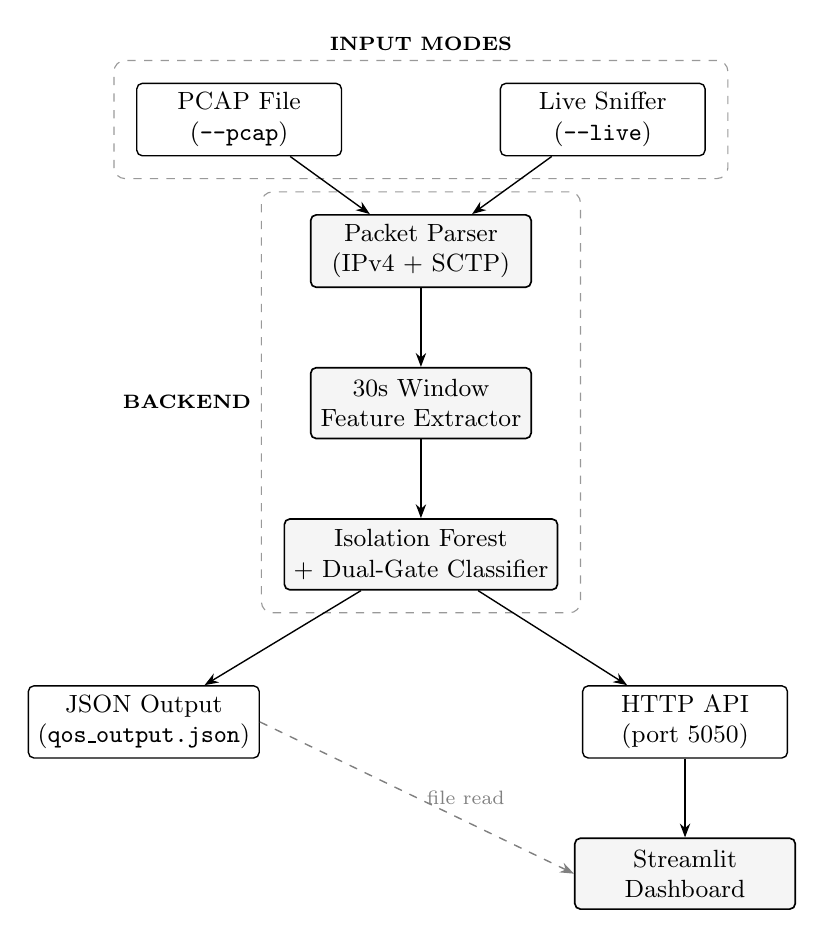
\begin{tikzpicture}[
    node distance=1.0cm and 1.5cm,
    every node/.style={font=\small},
    block/.style={rectangle, draw=black, fill=white, rounded corners=2pt,
                  minimum width=2.6cm, minimum height=0.9cm, align=center, line width=0.5pt},
    bigblock/.style={rectangle, draw=black, fill=gray!8, rounded corners=2pt,
                  minimum width=2.8cm, minimum height=0.9cm, align=center, line width=0.6pt},
    arr/.style={-{Stealth[length=5pt]}, line width=0.5pt, color=black},
    dasharr/.style={-{Stealth[length=5pt]}, line width=0.5pt, color=black!50, dashed},
    fitbox/.style={draw=black!40, dashed, rounded corners=4pt, inner sep=8pt, line width=0.4pt},
]

\node[block] (pcap) {PCAP File\\(\texttt{-{}-pcap})};
\node[block, right=2.0cm of pcap] (live) {Live Sniffer\\(\texttt{-{}-live})};

\node[bigblock, below=1.2cm of $(pcap)!0.5!(live)$] (parse) {Packet Parser\\(IPv4 + SCTP)};

\node[bigblock, below=1.0cm of parse] (window) {30s Window\\Feature Extractor};

\node[bigblock, below=1.0cm of window] (ml) {Isolation Forest\\+ Dual-Gate Classifier};

\node[block, below left=1.2cm and 0.3cm of ml] (json) {JSON Output\\(\texttt{qos\_output.json})};
\node[block, below right=1.2cm and 0.3cm of ml] (http) {HTTP API\\(port 5050)};

\node[bigblock, below=1.0cm of http] (dash) {Streamlit\\Dashboard};

\draw[arr] (pcap) -- (parse);
\draw[arr] (live) -- (parse);
\draw[arr] (parse) -- (window);
\draw[arr] (window) -- (ml);
\draw[arr] (ml) -- (json);
\draw[arr] (ml) -- (http);
\draw[arr] (http) -- (dash);
\draw[dasharr] (json.east) -- node[right, font=\scriptsize]{file read} (dash.west);

\begin{scope}[on background layer]
    \node[fitbox, fit=(pcap)(live), label={[font=\scriptsize\bfseries]above:INPUT MODES}] {};
    \node[fitbox, fit=(parse)(window)(ml), label={[font=\scriptsize\bfseries]left:BACKEND}] {};
\end{scope}

\end{tikzpicture}
\caption{System architecture. The backend supports offline PCAP analysis and live packet capture. Both modes produce identical JSON output consumed by the dashboard.}
\label{fig:arch}
\end{figure}

\subsection{Dual-Mode Input}

The backend supports two mutually exclusive input modes:

\begin{itemize}
    \item \textbf{PCAP mode} (\texttt{-{}-pcap}): Reads a recorded \texttt{.pcap} file using a custom binary parser (no external library dependency). Validates the pcap magic number and supports both little-endian and big-endian formats.
    \item \textbf{Live mode} (\texttt{-{}-live}): Spawns a background thread running a Scapy sniffer on a specified network interface (\texttt{-{}-iface}). Packets are buffered in a thread-safe \texttt{deque} and processed in rolling 30-second windows. An optional \texttt{-{}-duration} parameter controls capture length.
\end{itemize}

\subsection{5G Protocol Identification}

The parser identifies 5G control-plane protocols by mapping SCTP source and destination ports to known 3GPP interfaces:

\begin{table}[H]
\centering
\begin{tabular}{l l l}
\toprule
\textbf{Port} & \textbf{Interface} & \textbf{Protocol} \\
\midrule
38412 & N2 (AMF side)  & NGAP \\
38413 & N2 (gNB side)  & NGAP \\
38472 & F1-C (DU side) & F1AP \\
38473 & F1-C (CU side) & F1AP \\
\bottomrule
\end{tabular}
\caption{SCTP port-to-interface mapping for 5G control-plane protocol identification.}
\label{tab:ports}
\end{table}

Packets not matching any known port are classified as ``WiFi/Other''. The parser handles variable Ethernet header offsets and validates IPv4 version nibbles before extracting IP header length and total packet length.

% ══════════════════════════════════════════════════════════════════════════
\section{Feature Extraction}

Parsed packets are segmented into non-overlapping 30-second windows (configurable via \texttt{WINDOW\_SIZE}). Windows with fewer than 3 packets are discarded. For each valid window, eight QoS features are computed:

\begin{table}[H]
\centering
\begin{tabular}{l l p{7.5cm}}
\toprule
\textbf{Feature} & \textbf{Unit} & \textbf{Computation} \\
\midrule
Latency        & ms    & Mean inter-packet delay (IPD) within the window \\
Jitter         & ms    & Standard deviation of IPD \\
Throughput     & Mbps  & $\sum \text{pkt\_size} \times 8 \;/\; 30 \;/\; 10^6$ \\
Signal Strength & dBm  & Estimated as $-50 - (\text{loss\_rate} \times 60)$ \\
Resource Allocation & \%  & $(\text{delivered packets} / \text{total packets}) \times 100$, where delivered = total $-$ SACK gaps \\
Loss Rate      & ratio & Fraction of IPDs exceeding $5\times$ the median IPD \\
Burstiness     & ratio & $\max(\text{IPD}) / \text{mean}(\text{IPD})$ \\
Bandwidth Gap  & Mbps  & Per-window throughput minus the median throughput across all windows \\
\bottomrule
\end{tabular}
\caption{QoS features extracted per 30-second analysis window.}
\label{tab:features}
\end{table}

\subsection{SCTP SACK Gap Analysis}

A distinctive aspect of the feature extraction is the parsing of SCTP Selective Acknowledgement (SACK) chunks to estimate packet loss. The function \texttt{count\_sack\_gaps()} iterates over SCTP chunk headers, identifies SACK chunks (type \texttt{0x03}), and extracts the 16-bit gap count field at offset~+12. The total gap count per window is subtracted from the packet count to estimate successfully delivered packets, which feeds the Resource Allocation feature.

% ══════════════════════════════════════════════════════════════════════════
\section{ML Pipeline and Classification}

\subsection{Model Architecture}

The anomaly detection model uses \textbf{scikit-learn's Isolation Forest} with the following configuration:

\begin{table}[H]
\centering
\begin{tabular}{l l}
\toprule
\textbf{Parameter} & \textbf{Value} \\
\midrule
Algorithm         & Isolation Forest \\
Number of trees   & 100 (\texttt{n\_estimators}) \\
Contamination     & 0.10 (10\% expected anomaly rate) \\
Random state      & 42 (reproducibility) \\
Preprocessing     & StandardScaler (zero mean, unit variance) \\
\bottomrule
\end{tabular}
\caption{Isolation Forest model configuration.}
\label{tab:model}
\end{table}

The model is trained on four features: \texttt{signal\_strength\_dbm}, \texttt{latency\_ms}, \texttt{bw\_gap}, and \texttt{resource\_alloc\_pct}. These were selected as the primary indicators of QoS health, covering radio quality, delay performance, bandwidth adequacy, and delivery reliability respectively.

\subsection{Dual-Gate Classification}

A critical design choice is the \textbf{dual-gate classification} that combines the Isolation Forest output with rule-based thresholds. This addresses the well-known problem that unsupervised anomaly detectors alone produce excessive false positives in network telemetry.

The classification logic operates as follows:

\begin{enumerate}
    \item \textbf{Gate 1 --- Isolation Forest:} The model's \texttt{predict()} output flags a window as anomalous ($-1$) or normal ($+1$). The continuous \texttt{decision\_function()} score is retained for severity ranking.
    \item \textbf{Gate 2 --- Threshold validation:} An anomalous window is classified as ``QoS Degraded'' \emph{only if} at least one of three hard thresholds is breached:
    \begin{itemize}
        \item Latency $> 60$\,ms
        \item Resource Allocation $< 60\%$
        \item Bandwidth Gap $< 0$\,Mbps
    \end{itemize}
    \item \textbf{Three-state output:} Windows that are anomalous but do not breach any threshold are classified as ``Unusual but Acceptable'', avoiding unnecessary alerts.
\end{enumerate}

This AND-logic between Gates~1 and~2 substantially reduces false positive alerts compared to either method alone, while the third state (``Unusual but Acceptable'') provides early warning of emerging trends.

\begin{figure}[H]
\centering
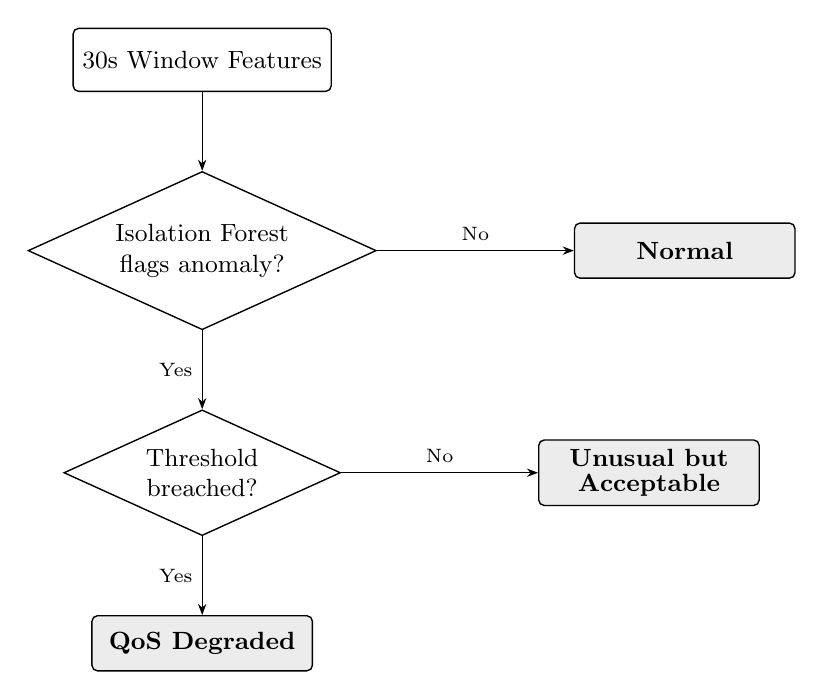
\begin{tikzpicture}[
    node distance=0.8cm,
    every node/.style={font=\small},
    block/.style={rectangle, draw=black, fill=white, rounded corners=2pt,
                  minimum width=3.2cm, minimum height=0.8cm, align=center, line width=0.5pt},
    decision/.style={diamond, draw=black, fill=white, aspect=2.2,
                     minimum width=2cm, align=center, line width=0.5pt, font=\small},
    result/.style={rectangle, draw=black, fill=gray!15, rounded corners=2pt,
                   minimum width=2.8cm, minimum height=0.7cm, align=center, line width=0.5pt},
    arr/.style={-{Stealth[length=4pt]}, line width=0.4pt},
]

\node[block] (input) {30s Window Features};
\node[decision, below=1.0cm of input] (g1) {Isolation Forest\\flags anomaly?};
\node[result, right=2.5cm of g1] (normal) {\textbf{Normal}};
\node[decision, below=1.0cm of g1] (g2) {Threshold\\breached?};
\node[result, right=2.5cm of g2] (unusual) {\textbf{Unusual but}\\[-2pt]\textbf{Acceptable}};
\node[result, below=1.0cm of g2] (degraded) {\textbf{QoS Degraded}};

\draw[arr] (input) -- (g1);
\draw[arr] (g1) -- node[above, font=\scriptsize]{No} (normal);
\draw[arr] (g1) -- node[left, font=\scriptsize]{Yes} (g2);
\draw[arr] (g2) -- node[above, font=\scriptsize]{No} (unusual);
\draw[arr] (g2) -- node[left, font=\scriptsize]{Yes} (degraded);

\end{tikzpicture}
\caption{Dual-gate classification flowchart. The three-state output distinguishes genuine degradation from benign anomalies.}
\label{fig:dualgate}
\end{figure}

% ══════════════════════════════════════════════════════════════════════════
\section{Output and Dashboard Integration}

\subsection{JSON Output Schema}

The backend produces a structured JSON payload with three top-level keys:

\begin{itemize}
    \item \textbf{\texttt{sessions}}: Array of per-window records containing all extracted features, anomaly score, and QoS status. Fields are renamed for dashboard compatibility (e.g., \texttt{Signal\_Strength\_dBm}, \texttt{Latency\_ms}, \texttt{QoS\_Status}).
    \item \textbf{\texttt{summary}}: Aggregate statistics including total sessions, counts per QoS state, degradation rate percentage, and mean values for latency, signal strength, and resource allocation.
    \item \textbf{\texttt{alerts}}: Degraded windows sorted by anomaly score (worst first), providing a prioritised alert queue.
\end{itemize}

\subsection{HTTP API}

The backend optionally starts a lightweight HTTP server (port 5050, configurable via \texttt{-{}-port}) that serves the JSON payload via \texttt{GET /}. CORS headers are included for browser-based dashboard consumption. In live mode, the payload is refreshed every 30 seconds as new windows are analysed.

\subsection{Real-Time Dashboard}

The Streamlit dashboard consumes the JSON output and provides:

\begin{itemize}
    \item Summary cards showing total sessions, degradation rate, and aggregate QoS metrics.
    \item Time-series area charts for latency, jitter, signal strength, throughput, and burstiness.
    \item Colour-coded QoS status indicators per window.
    \item Alert panel listing degraded windows sorted by severity.
    \item One-click CSV export for post-incident forensic analysis.
\end{itemize}

% ══════════════════════════════════════════════════════════════════════════
\section{5G Network Capabilities Utilised}

The solution is designed to exploit native 5G capabilities:

\begin{table}[H]
\centering
\begin{tabular}{l p{9.8cm}}
\toprule
\textbf{Capability} & \textbf{Role in the Monitoring Pipeline} \\
\midrule
eMBB           & High-throughput telemetry ingestion from concurrent UEs at sub-second granularity \\
URLLC          & End-to-end inference loop (capture $\to$ prediction $\to$ alert) within a single 30s window cycle \\
Network Slicing & Dedicated monitoring slice isolates telemetry traffic from user-plane data \\
MEC            & Backend deployment at edge node co-located with gNodeB for low-latency inference \\
QoS Framework  & 5QI-based flow prioritisation for telemetry streams; GBR bearers ensure lossless alert delivery \\
\bottomrule
\end{tabular}
\caption{5G-native capabilities and their role in the monitoring pipeline.}
\label{tab:5gcap}
\end{table}

% ══════════════════════════════════════════════════════════════════════════
\section{Scalability and Market Readiness}

\subsection{Architecture}

The system is designed for horizontal scalability:

\begin{itemize}
    \item The backend is stateless in PCAP mode; multiple instances can process different capture files concurrently.
    \item In live mode, the thread-safe \texttt{deque} buffer and periodic processing loop enable continuous operation without memory growth.
    \item The lightweight HTTP server (stdlib-based, no framework dependency) adds minimal overhead.
    \item The Isolation Forest model ($<$5\,MB serialised) has sub-linear inference time $O(n \log \psi)$, enabling real-time scoring.
\end{itemize}

\subsection{Deployment}

The system requires only standard Python packages (\texttt{scikit-learn}, \texttt{pandas}, \texttt{numpy}, \texttt{scapy}) and can be containerised as a single Docker image. No GPU is required. Deployment scenarios include:

\begin{table}[H]
\centering
\begin{tabular}{l p{9cm}}
\toprule
\textbf{Sector} & \textbf{Application} \\
\midrule
Smart Manufacturing & Monitoring AGVs, robotic arms, and vision systems on private 5G factory floors \\
Healthcare          & QoS assurance for remote surgery and real-time patient monitoring \\
Ports and Logistics & Crane automation and fleet management over private 5G \\
Smart Campuses      & Enterprise networks with dense IoT and AR/VR workloads \\
Disaster Management & First-responder communication on portable 5G cells \\
\bottomrule
\end{tabular}
\caption{Target deployment sectors.}
\label{tab:sectors}
\end{table}

\subsection{Business Model}

\begin{itemize}
    \item \textbf{SaaS:} Per-site, per-month monitoring subscription.
    \item \textbf{Enterprise License:} On-premise perpetual license for defence and critical infrastructure.
    \item \textbf{Consulting:} Custom PCAP forensics, model retraining on domain-specific data, and compliance audits.
\end{itemize}

% ══════════════════════════════════════════════════════════════════════════
\section{Societal and Industrial Impact}

\begin{table}[H]
\centering
\begin{tabular}{l c c}
\toprule
\textbf{Metric} & \textbf{Legacy NMS} & \textbf{Our System} \\
\midrule
Mean-Time-To-Detect           & 5--15 min       & $<$ 30\,s (one window) \\
False Positive Rate            & 18--25\%        & Reduced via dual-gate \\
Post-Incident Forensic Time    & 4--8 hours      & Minutes (automated PCAP) \\
Classification Granularity     & Binary          & Three-state \\
\bottomrule
\end{tabular}
\caption{Operational improvement over legacy monitoring.}
\label{tab:impact}
\end{table}

\subsection{Alignment with National Initiatives}

\begin{itemize}
    \item \textbf{100 5G Use Case Labs Initiative:} Contributes a reusable, open-architecture monitoring toolkit for private 5G testbeds.
    \item \textbf{Make in India:} Indigenously developed solution reducing dependence on imported NMS platforms.
    \item \textbf{National Telecom Policy 2024:} Supports the policy's emphasis on AI-driven network automation and predictive maintenance.
    \item \textbf{Digital India:} Enables confident private 5G adoption in Tier-2 and Tier-3 cities through affordable, automated QoS monitoring.
\end{itemize}

% ══════════════════════════════════════════════════════════════════════════
\section{Novelty}

\begin{table}[H]
\centering
\begin{tabular}{p{3cm} p{4.5cm} p{4.5cm}}
\toprule
\textbf{Aspect} & \textbf{Existing Approaches} & \textbf{Our Innovation} \\
\midrule
Detection        & Static thresholds or supervised models requiring labelled data & Unsupervised Isolation Forest---no labelled failure data needed \\
Classification   & Binary (normal/alarm) & Three-state dual-gate: Normal, Unusual but Acceptable, QoS Degraded \\
Protocol Awareness & Generic IP/TCP analysis & 5G-specific SCTP port mapping (NGAP, F1AP) and SACK gap parsing \\
Mode Flexibility & Offline-only or online-only tools & Unified dual-mode backend with identical output schema \\
Deployment       & Heavy NMS platforms & Single Python script; no GPU; stdlib HTTP server \\
\bottomrule
\end{tabular}
\caption{Novelty comparison.}
\label{tab:novelty}
\end{table}

\subsection{Intellectual Property Potential}

\begin{itemize}
    \item \textbf{Patent-eligible:} Dual-gate three-state anomaly classification combining unsupervised ML with rule-based validation for 5G QoS assurance.
    \item \textbf{Copyright:} SCTP SACK gap-based loss estimation pipeline and per-window QoS feature schema.
\end{itemize}

% ══════════════════════════════════════════════════════════════════════════
\section{Deliverables}

\begin{table}[H]
\centering
\begin{tabular}{c l p{7cm} c}
\toprule
\textbf{\#} & \textbf{Deliverable} & \textbf{Description} & \textbf{Status} \\
\midrule
D1 & Backend Engine & Dual-mode Python backend with PCAP parsing, live capture, feature extraction, ML pipeline, and HTTP API & Complete \\
D2 & Dashboard & Streamlit real-time dashboard with charts, alerts, and CSV export & Complete \\
D3 & Trained Model & Isolation Forest (100 trees, 10\% contamination) with StandardScaler & Complete \\
D4 & JSON Schema & Documented output schema with sessions, summary, and alerts & Complete \\
D5 & Performance Report & Latency, accuracy, and stress-test benchmarks & In Progress \\
\bottomrule
\end{tabular}
\caption{Project deliverables.}
\label{tab:deliverables}
\end{table}

% ══════════════════════════════════════════════════════════════════════════
\section{Implementation Roadmap}

\begin{table}[H]
\centering
\begin{tabular}{l p{8cm} l}
\toprule
\textbf{Phase} & \textbf{Activities} & \textbf{Timeline} \\
\midrule
Proposal       & Submission and initial prototype demo & Mar--Apr 2026 \\
Validation     & National-level presentation; live demo at TEC & May--Jun 2026 \\
Pragati        & Mentor-guided hardening; integration with 5G testbed; model retraining on live data; dashboard UX refinement & Jun--Sep 2026 \\
Demonstration  & Physical demonstration before TEEC; stress testing & Sep 2026 \\
Showcase       & Awards and showcase at India Mobile Congress 2026 & Oct 2026 \\
\bottomrule
\end{tabular}
\caption{Project implementation roadmap.}
\label{tab:roadmap}
\end{table}

% ══════════════════════════════════════════════════════════════════════════
\section{Evaluation Criteria Mapping}

\begin{table}[H]
\centering
\begin{tabular}{l c p{8cm}}
\toprule
\textbf{Criterion} & \textbf{Weight} & \textbf{How We Address It} \\
\midrule
Technical Execution & 40\% & Working dual-mode backend with PCAP parsing, SCTP analysis, Isolation Forest pipeline, dual-gate classifier, and HTTP API serving real-time JSON \\
Scalability, Market Readiness & 40\% & Single-script deployment; no GPU; Docker-ready; vendor-agnostic; SaaS business model; five target verticals \\
Societal, Industrial Impact & 10\% & Healthcare, agriculture, disaster management; Digital India and Make in India alignment; Tier-2/3 city enablement \\
Novelty & 10\% & Three-state dual-gate classification; SCTP SACK gap analysis; unified online/offline architecture; 5G protocol awareness \\
\bottomrule
\end{tabular}
\caption{Evaluation criteria mapping.}
\label{tab:criteria}
\end{table}

% ══════════════════════════════════════════════════════════════════════════
\section{Video Demonstration}

A complete video demonstration of the working prototype, illustrating the real-time QoS monitoring dashboard, anomaly detection pipeline, and live 5G packet analysis workflow, can be found at the following link:

\begin{center}
\large
\href{https://drive.google.com/file/d/1o2JeBPJFspz6Ibny3hdDM3Wm70WVnwAe/view?usp=sharing}{\textbf{Watch the Video Demonstration Here}}
\end{center}

% ══════════════════════════════════════════════════════════════════════════
\section{References}

\begin{enumerate}[label={[\arabic*]}, leftmargin=2em, itemsep=3pt]
    \item 3GPP TS 23.501, ``System Architecture for the 5G System,'' Release 18, 2024.
    \item 3GPP TS 28.552, ``Management and Orchestration; 5G Performance Measurements,'' Release 18, 2024.
    \item 3GPP TS 38.413, ``NG Application Protocol (NGAP),'' Release 18, 2024.
    \item 3GPP TS 38.473, ``F1 Application Protocol (F1AP),'' Release 18, 2024.
    \item ETSI GS MEC 011, ``Multi-access Edge Computing; MEC Platform Application Enablement,'' V3.2.1, 2023.
    \item F.~T. Liu, K.~M. Ting, and Z.-H. Zhou, ``Isolation Forest,'' in \emph{Proc. IEEE ICDM}, 2008, pp.~413--422.
    \item RFC 4960, ``Stream Control Transmission Protocol,'' IETF, 2007.
    \item DoT India, ``National Telecom Policy 2024,'' Government of India, 2024.
    \item DoT India, ``100 5G Use Case Labs Initiative --- Guidelines and Framework,'' 2025.
\end{enumerate}

% ── Footer ────────────────────────────────────────────────────────────────
\vspace{12pt}
\noindent\rule{\textwidth}{0.8pt}
\begin{center}
    \small\itshape
    AI-Driven Private 5G QoS Monitor $\cdot$ Use Case Report $\cdot$ April 2026
\end{center}

\end{document}